\documentclass[]{article}
\usepackage[a4paper, total={6in, 8in}]{geometry}
\usepackage[autostyle]{csquotes}
\usepackage[utf8]{inputenc}
\usepackage{booktabs}
\usepackage[backend=bibtex]{biblatex}
\bibstyle{abbrv}
\addbibresource{bibliography}

\usepackage{tikz}
\usetikzlibrary{calc}
\usetikzlibrary{shapes.geometric, arrows, fit}

\tikzstyle{process} = [rectangle, 
minimum width=12cm, 
minimum height=1cm, 
text width=11cm, 
draw=black, 
fill=white,
rounded corners]

\tikzstyle{subprocess} = [rectangle, 
minimum width=5cm, 
minimum height=0.6cm, 
text centered, 
text width=5cm, 
draw=black, 
fill=white]

\tikzstyle{lsnode} = [rectangle, 
minimum width=2cm, 
minimum height=0.6cm, 
text centered, 
text width=2cm, 
draw=black, 
fill=white]

\tikzstyle{arrow} = [thick,->,>=stealth]
\tikzstyle{dashedarrow} = [dashed,->,>=stealth]

\begin{document}
\section{Introduction}
Electrification  of public transport has become the norm over recent years. Many public transport poviders, such as the Dutch bus provider Qbuzz \cite{qbuzzQbuzz}, have been electrifying their fleet with the aim of reducing their carbon footprint in order to match the stricter regulations set out by organizations such as the European Union \cite{europaRegulation20181999}. This electrification introduces new challenges in every step of the planning process as seen in Figure \ref{fig:planning-overview}, as the limits of both electric infrastructure and electric vehicles add new constraints to an already complex operation. Existing techniques that minimize operational costs therefore need to be revised in order to add consideration for these new constraints. \\\\
In this work, we will focus on two of the most costly steps of the planning process for busses: vehicle and crew scheduling TODO: citation needed. When considered seperately (refered to as a sequential approach), these problems are often refered to as the Vehicle Scheduling Problem (VSP) and Crew Scheduling Problem (CSP). When considered together (refered to as an integrated approach), this becomes the Vehicle and Crew Scheduling Problem (VCSP). \\\\
A lot of work has already been for these problems. Both the sequential and integrated approach have been extensively studied since the 1980s, and we refer the reader to a recent survey in order to get a sense of the current state of the art TODO: citiation met survey. The introduction of electric vehicles has however introduced some new problems. The most important of these are the limited range of these vehicles, as well as charging times which greatly exceed the refueling times found in traditional combustion based busses. This most directly effects the VSP, as charging periods now need to be added throughout the day in order to effectively use a bus. This new version of the problem, refered to as the E-VSP (as well as E-CSP and E-VCSP for the other problems respectively) has also been studied in the past. We once again refer the reader to a recent survey in order to get a better understanding of the current work. \\\\
Most work using electric vehicles up until now has focused on the sequential approach. This leaves some room for improvement, as was already pointed out back in the 1980s \cite{RAFF198363}. This is largely attributed to the fact that costs associated with crew assignment often dominate those for vehicle assignment; it is therefore potentially adventagous to include crew considerations during the vehicle planning step in order to reduce costs. \\\\
Some literature does exist on the E-VSCP problem, however some simplifying assumptions are made which might limit real world applicability or accurate modeling of costs. Most notably, assumptions are made about charging locations (such as only being able to charge at a bus depot), charging behavior (such as modeling the process as being purely linear or only allowing full charges). Additionally, to the best of our knowledge battery degredation has not been included in any integrated models at the time of writing. The contribution of this work is therefore threefold: 
\begin{itemize}
  \item Including more flexible battery constraints by allowing partial charging at locations other than a depot while taking into account time based electricity prices. 
  \item Including battery degredation into the objective function.
  \item Using lagrangian relaxation instead of currently used methods as a basis for the solution method. 
\end{itemize}
\begin{figure}[h]
\centering
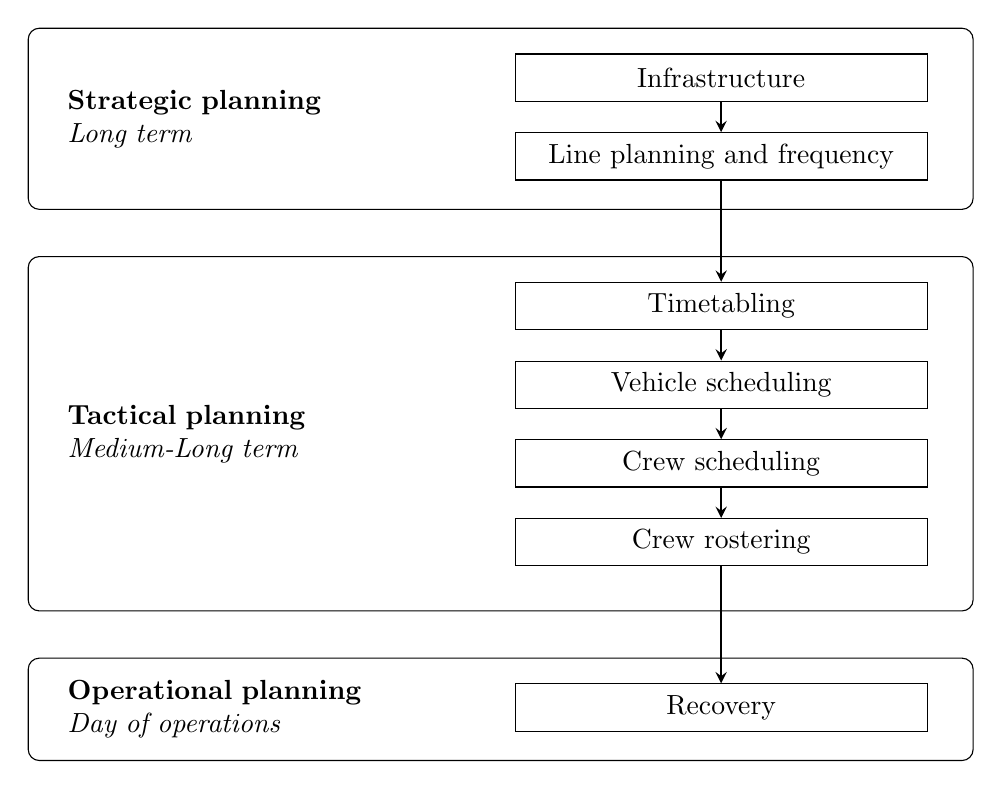
\begin{tikzpicture}[node distance=2cm]
  \node (strategic) [process, minimum height=2.3cm] {\textbf{Strategic planning}\\\textit{Long term}};
  \node at (strategic.base) (infra) [subprocess, xshift=2.8cm, yshift=0.4cm] {Infrastructure};
  \node at (strategic.base) (line) [subprocess, below of=infra, yshift=1cm] {Line planning and frequency};
  
  \node (tactical) [process, minimum height=4.5cm, below of=strategic, yshift=-2cm] {\textbf{Tactical planning}\\\textit{Medium-Long term}};
  \node at (tactical.base) (timetable) [subprocess, xshift=2.8cm, yshift=1.5cm] {Timetabling};
  \node at (tactical.base) (vehicle) [subprocess, below of=timetable, yshift=1cm] {Vehicle scheduling};
  \node at (tactical.base) (crew) [subprocess, below of=vehicle, yshift=1cm] {Crew scheduling};
  \node at (tactical.base) (rostering) [subprocess, below of=crew, yshift=1cm] {Crew rostering};

  \node (operational) [process, minimum height=1.3cm, below of=tactical, yshift=-1.5cm] {\textbf{Operational planning}\\\textit{Day of operations}};
  \node at (operational.base) (recovery) [subprocess, xshift=2.8cm, yshift=-0.1cm] {Recovery};


  \draw [arrow] (infra) -- (line);
  \draw [arrow] (line) -- (timetable);
  \draw [arrow] (timetable) -- (vehicle);
  \draw [arrow] (vehicle) -- (crew);
  \draw [arrow] (crew) -- (rostering);
  \draw [arrow] (rostering) -- (recovery);
\end{tikzpicture}
\caption{A general overview of the public transport planning process, based on \cite{IBARRAROJAS201538}, \cite{PERUMAL2022395}.}
\label{fig:planning-overview}
\end{figure}


\section{Related work}
For an introduction to lagrangian relaxation, we refer the reader to a general overview by Beasley \cite{Beasley1993}. Lagrangian relaxation has already succesfully been applied to the VSCP problem; examples  \\\\
As far as we are aware, only four other works discuss the electric integrated vehicle and crew scheduling problem (E-VCSP). Perumal et al. introduced an adaptive large neighbourhood search (ALNS) approach to the problem in 2021 \cite{PERUMAL2021105268}. They only consider full recharges, charging at the depot and fixed maximum ranges for vehicles. Sistig and Sauer also offered a ALNS based approach in 2023, which aimed to include partial, opportunisitic charging and more \cite{SISTIG2023120915}. Wang et al. introduce a two layered model using particle swarms and a $\epsilon$-constraint based mechanism which allows for a mix of diesel and electric busses, which incorporates partial depot charging \cite{su14063627}.
Shen and Li provide a minimum-cost flow based approach to solving the problem, incorporating interesting driving time considerations. They only provide full recharge capabilities. \cite{SHEN2023}

\begin{table}[h]
  \centering
  \begin{tabular}{cllllll}
      \toprule
      & Model & TOU & SoC & Partial charging & Charge location & Degredation \\
      \cmidrule(lr){2-7}
      \cite{PERUMAL2021105268} & VSCP & ? & ? & No & Depot & No  \\
      \cite{SISTIG2023120915} & VSCP & ? & ? & Yes & ? & No \\
      \cite{su14063627} & VSCP & Yes & C & Yes & Depot & No \\
      \cite{SHEN2023} & VSCP & ? & ? & No & ? & No \\
      \bottomrule
  \end{tabular}
  \caption{Overview of battery modeling in E-VSP and E-VSCP literature. TOU = time of use electricity prices, State of charge (SoC) is either modeled as a (D)iscrete or (C)ontinuous variable}
  \label{tab:evscp-lit}
\end{table}

\printbibliography
\end{document}